% ============================================================
% cmsimile: three approaches to scoring relatedness of sub-families A and B.
%
% LAYOUT (relative): nothing in the main picture has a hand-typed position.
%   - a "Setup" frame sits at the origin; everything inside it is chained
%     (tree -> text to its right -> definitions below that).
%   - three fixed-size panel frames c1, c2, c3 sit below it, side by side.
%   - inside each panel, blocks are stacked top-to-bottom with
%       \node[stack={previous}{gap}] (name) {...};
%     and the output box is pinned to the bottom of its frame.
%   Every block (Venn, tree, plots) is its own little tikzpicture with a
%   fixed size in mm (y points down), so it behaves like a single box.
% To add a line/block: insert a new \node[stack=...] and re-point the
% node after it at the new one. Raise \panelh if a panel gets too full.
% ============================================================
\documentclass[tikz,border=4pt]{standalone}
\usepackage[T1]{fontenc}
\renewcommand{\familydefault}{\sfdefault}
\usepackage{sansmath}
\usepackage{xcolor}
\usetikzlibrary{arrows.meta,calc,positioning,fit,backgrounds,matrix}

% ============================================================
% Shared style definitions for the DarwinsRNAHunt methods figures.
% \input this file from each diagram's preamble (after \usepackage{xcolor}
% and \usetikzlibrary{...}) so colours/styles stay consistent everywhere.
%
% Visual grammar used throughout:
%   - white box, single border   = external / raw resource
%   - white box, double border   = curated data artifact (output of a section)
%   - coloured box, single border = an internal processing step
%   - coloured/white, dashed border = Snakemake checkpoint (dynamic re-evaluation)
%   - white box, short-dashed border = static external file (not produced by the pipeline)
% ============================================================

% ---------- category colours (ColorBrewer Set3-style) ----------
\definecolor{catDefine}{HTML}{FFFFFF}
\definecolor{catSelect}{HTML}{FFFFFF}
\definecolor{catAcquire}{HTML}{FFFFFF}
\definecolor{catLocalize}{HTML}{FFFFFF}
\definecolor{catExtract}{HTML}{FFFFFF}
\definecolor{catCombine}{HTML}{FFFFFF}
\definecolor{catCluster}{HTML}{FFFFFF}
\definecolor{catModel}{HTML}{FFFFFF}
\definecolor{catValidate}{HTML}{FFFFFF}
\definecolor{catReport}{HTML}{FFFFFF}

% ---------- Kea Palette (defined for optional future restyling; unused for now) ----------
\definecolor{keaGreen}{HTML}{6C803A}
\definecolor{darkBrown}{HTML}{7B5C34}
\definecolor{lightBrown}{HTML}{AB7C47}
\definecolor{keaYellow}{HTML}{CCAE42}
\definecolor{keaOrange}{HTML}{D73202}
\definecolor{charcoal}{HTML}{272318}
\definecolor{lightGrey}{HTML}{D3CDBF}

\tikzset{
    font=\fontsize{7}{8}\selectfont,
    >={Latex[length=2mm,width=1.4mm]},
    every path/.style={thick},
    % internal processing step
    stage/.style={rectangle, rounded corners=2pt, draw=black, thin,
        minimum height=1.05cm, text width=3.6cm, align=center, inner sep=3pt},
    % external / raw resource (input)
    res/.style={rectangle, rounded corners=2pt, draw=black, thin, fill=white,
        minimum height=1cm, text width=4.2cm, align=center, inner sep=3pt},
    % static external file, not produced by this pipeline
    ext/.style={rectangle, rounded corners=2pt, draw=black!55, dash pattern=on 2.2pt off 1.6pt,
        thin, minimum height=0.85cm, text width=3.1cm, align=center, fill=white,
        font=\fontsize{6.3}{7.3}\selectfont, inner sep=2.5pt},
    % Snakemake checkpoint modifier (combine with stage/res)
    ckpt/.style={dashed, line width=0.9pt},
    % deliverable / output-artifact modifier: crosses a section boundary
    deliver/.style={double, double distance=1.2pt, line width=0.85pt},
    lbl/.style={font=\fontsize{8.5}{9.5}\bfseries\selectfont},
    sublbl/.style={font=\fontsize{7}{8}\itshape\selectfont},
    node distance=0.55cm and 2.6cm
}
   % shared DarwinsRNAHunt style sheet (change name/path if needed)

% ---------- colours for this figure ----------
\colorlet{colA}{keaOrange}
\colorlet{colB}{keaYellow}              % change here to recolour B everywhere
\colorlet{colOverlap}{keaGreen}
\colorlet{nullGrey}{charcoal!45}

% ---------- page geometry ----------
\newlength{\panelw}  \setlength{\panelw}{57mm}     % panel width
\newlength{\panelgap}\setlength{\panelgap}{3.5mm}  % gap between panels
\newlength{\panelh}  \setlength{\panelh}{93mm}     % panel height (raise if a panel overflows)
\newlength{\padding} \setlength{\padding}{2mm}     % padding inside every frame
\newlength{\innerw}  \setlength{\innerw}{\dimexpr\panelw-2\padding\relax}  % = 53mm: width of every block
\newlength{\totw}    \setlength{\totw}{\dimexpr3\panelw+2\panelgap\relax}

% ---------- text macros ----------
\newcommand{\cA}{\textcolor{colA}{\textbf{A}}}
\newcommand{\cB}{\textcolor{colB}{\textbf{B}}}
\newcommand{\mobs}{m_{\mathrm{obs}}}
\newcommand{\shuf}{\texttt{dinucshuffle}}   % name of the dinucleotide shuffle function

\def\xmin{-0.35}   % left edge of the bit-score axis (panels 1 and 3)
\def\xmax{1.05}

\newcommand{\xpos}[1]{\L+\Wd*((#1)-(\xmin))/(\xmax-\xmin)}

\tikzset{
  blk/.style={x=1mm, y=-1mm, color=charcoal},        % local system inside a block: mm, y down
  stack/.style 2 args={below=#2 of #1.south west, anchor=north west, inner sep=0pt},
  panel/.style={draw=lightGrey!85!charcoal, line width=.5pt, rounded corners=1mm}, % use draw=none to hide frames
  col/.style={panel, minimum width=\panelw, minimum height=\panelh, inner sep=0pt},
  txt/.style={anchor=base west, inner sep=0pt},
  ctr/.style={anchor=base, inner sep=0pt},
  bigA/.style={font=\fontsize{9}{10}\bfseries\selectfont},
  axis/.style={line width=0.5pt},
  outbox/.style={res, deliver, text width=48mm, minimum height=8mm, inner sep=2pt},
  procstep/.style={stage, fill=white, minimum height=4.8mm, inner sep=1pt}
}
\newcommand{\bbox}[2]{\useasboundingbox (0,0) rectangle (#1,#2);}

% ---------- logistic curves for the score distributions ----------
% (z clamped to +-8 to stay inside pgfmath's fixed-point range)
\pgfmathdeclarefunction{lgc}{3}{% cdf(x, mean, scale)
  \pgfmathparse{1/(1+exp(-max(min(((#1)-(#2))/(#3),8),-8)))}}
\pgfmathdeclarefunction{lgp}{3}{% pdf(x, mean, scale)
  \pgfmathparse{lgc(#1,#2,#3)*(1-lgc(#1,#2,#3))/(#3)}}
% null: narrow, long right tail (mixture).  observed: wider, shifted right.
\newcommand{\nullcdf}[1]{(0.7*lgc(#1,0.42,0.030)+0.3*lgc(#1,0.56,0.077))}
\newcommand{\nullpdf}[1]{(0.7*lgp(#1,0.42,0.030)+0.3*lgp(#1,0.56,0.077))}
\newcommand{\obscdf}[1]{lgc(#1,0.66,0.094)}
\newcommand{\obspdf}[1]{lgp(#1,0.66,0.094)}
\def\xmed{0.66}    % median of the observed curve
\def\xD{0.52}      % x of the largest CDF gap; recompute if you change the parameters
\def\dscale{2.30}  % mm of density height per unit pdf (null peak = 14.5 mm)

% ---------- helpers ----------
% \elbow{child1}{child2}{y of join}{name of new node}{colour}   (inside a block)
\newcommand{\elbow}[5]{%
  \draw[#5] (#1) -- (#1 |- 0,#3) -- (#2 |- 0,#3) -- (#2);
  \path (#1) -- (#2) coordinate[pos=.5] (tmp);
  \coordinate (#4) at (tmp |- 0,#3);}

% panel header, pinned to the top-left of frame #1: nodes #1-h (title)
\newcommand{\panelhead}[3]{%
  \node[anchor=north west, inner sep=0pt] (#1-h) at ([shift={(\padding,-\padding)}]#1.north west)
    {{\fontsize{10}{11}\bfseries\selectfont #2}};
  \node[stack={#1-h}{0.8mm}, sublbl] (#1-s) {#3};}

% Venn block (53 x 16.5 mm); #1 name, #2 node above, #3 gap, #4 extra drawing (e.g. \adots)
\newcommand{\vennblock}[4]{%
  \node[stack={#2}{#3}] (#1) {\begin{tikzpicture}[blk]
    \bbox{53}{16.5}
    \fill[colA, opacity=.13] (21.5,8.4) circle[radius=7.6mm];
    \fill[colB, opacity=.13] (31.6,8.4) circle[radius=7.6mm];
    \begin{scope}[every path/.style={}]  % the shared sheet's 'thick' would break \clip
      \clip (21.5,8.4) circle (7.6mm);
      \fill[colOverlap, opacity=.6] (31.6,8.4) circle[radius=7.6mm];
    \end{scope}
    \draw[colA, line width=.7pt] (21.5,8.4) circle[radius=7.6mm];
    \draw[colB, line width=.7pt] (31.6,8.4) circle[radius=7.6mm];
    \node[ctr, bigA, text=colA] at (13.2,2.6) {A};
    \node[ctr, bigA, text=colB] at (39.9,2.6) {B};
    #4
  \end{tikzpicture}};}
\newcommand{\adots}{%   % sequences a_i drawn as dots in A
  \foreach \dx/\dy in {-4.8/-2.5, -5.8/1.0, -3.8/3.6, -1.9/-4.3, -1.5/0.8}
    \fill[colA] ({21.5+\dx},{8.4+\dy}) circle[radius=.53mm];}

\begin{document}
\sansmath
\begin{tikzpicture}

% ================================================================= SETUP
\coordinate (S0) at (0,0);
\coordinate (SR) at (\totw,0);
% \node[anchor=north west, inner sep=0pt, lbl] (setuplbl) at ([shift={(\padding,-\padding)}]S0) {Let};

% tree of R with sub-families A and B (block, 50 x 29 mm)
\node[anchor=north west] at ([shift={(\padding,-\padding)}]S0) (tree) {\begin{tikzpicture}[blk]
  \bbox{50}{29}
  \begin{scope}[shift={(-4,-6)}]
    \fill[colA, opacity=.12, rounded corners=1mm] (5.6,16.8) rectangle (19.8,27.2);
    \fill[colB, opacity=.12, rounded corners=1mm] (38.6,16.8) rectangle (52.8,27.2);
    \coordinate (a1) at (7.6,25.4);  \coordinate (a2) at (12.7,25.4); \coordinate (a3) at (17.8,25.4);
    \coordinate (g1) at (25.4,25.4); \coordinate (g2) at (30.5,25.4);
    \coordinate (b1) at (40.6,25.4); \coordinate (b2) at (45.7,25.4); \coordinate (b3) at (50.8,25.4);
    \elbow{a1}{a2}{21.8}{nA1}{colA}
    \elbow{nA1}{a3}{18.5}{nA2}{colA}
    \elbow{g1}{g2}{22.1}{nG}{nullGrey}
    \elbow{b1}{b2}{21.8}{nB1}{colB}
    \elbow{nB1}{b3}{18.5}{nB2}{colB}
    \elbow{nG}{nB2}{14.2}{nR1}{charcoal}
    \elbow{nA2}{nR1}{10.7}{root}{charcoal}

    \coordinate (rr) at (8.8,10.7);
    \fill[nullGrey, opacity=.25] (rr) -- (5.6,15.4) -- (12.0,15.4) -- cycle;
    \draw[nullGrey] (rr) -- (5.6,15.4) -- (12.0,15.4) -- cycle;
    \elbow{rr}{root}{9.4}{rootR}{charcoal}
    \node[ctr, text=nullGrey, font=\fontsize{7}{8}\itshape\selectfont] at (rr |- 0,7.7) {rest of R};

    \draw (rootR) -- (rootR |- 0,8.4);
    \node[ctr, font=\fontsize{8}{9}\bfseries\itshape\selectfont] at (rootR |- 0,7.4) {R};

    \foreach \p/\c in {a1/colA,a2/colA,a3/colA,g1/nullGrey,g2/nullGrey,b1/colB,b2/colB,b3/colB}
    \fill[\c] (\p) circle[radius=.57mm];
    \foreach \p/\n in {a1/1,a2/2,a3/3}
    \node[ctr, text=colA, font=\fontsize{7}{8}\itshape\selectfont] at (\p |- 0,29) {$a_\n$};
    \foreach \p/\n in {b1/1,b2/2,b3/3}
    \node[ctr, text=colB, font=\fontsize{7}{8}\itshape\selectfont] at (\p |- 0,29) {$b_\n$};
    \draw[colA, line width=.6pt] (6.6,30.5) -- (18.8,30.5);
    \draw[colB, line width=.6pt] (39.6,30.5) -- (51.8,30.5);
    \node[ctr, bigA, text=colA] at (12.7,33.7) {A};
    \node[ctr, bigA, text=colB] at (45.7,33.7) {B};
  \end{scope}
\end{tikzpicture}};

% text to the right of the tree, chained downwards
\node[right=6mm of tree.north east, anchor=north west, inner sep=0pt] (n1)
  {\cA{} and \cB{} are models describing similar and related RNA families within a larger space of all };
\node[stack={n1}{1.6mm}] (n2)
  {RNA sequences, $$R$$.};
\node[stack={n2}{1.6mm}] (n3)
  {Sequences $a_i$ are members of \cA; sequences $b_i$ are members of \cB};
% function definitions: two aligned columns (add a row for each new function)
\matrix (defs) [stack={n3}{2.2mm}, matrix of nodes, ampersand replacement=\&,
                nodes={anchor=base west, inner sep=0pt}, column sep=3mm, row sep=1.3mm] {
  \textbf{\texttt{cmemit(A)}}      \& $\rightarrow$ set of sequences, members of $A$ \\
  \textbf{\texttt{cmsearch($a_i$, B)}} \& $\rightarrow$ log-odds bit score that $a_i$ is part of $B$ \\
  \textbf{\texttt{dinucshuffle($a_i$)}} \& $\rightarrow$ random sequence set with the same dinucleotide counts as $a_i$ \\
};
\node[stack={defs}{2.2mm}, font=\fontsize{8}{9}\bfseries\selectfont] (q) {How related are \cA{} and \cB{}?};

% frame around the setup, full page width, grows with its contents
\coordinate (padL) at ($(tree.south west)+(0,-\padding)$);
\coordinate (padR) at ($(q.south west)+(0,-\padding)$);
\begin{scope}[on background layer]
  \node[panel, inner sep=0pt, fit=(S0)(SR)(tree)(q)(padL)(padR)] (setupbox) {};
\end{scope}

% ================================================================= PANEL FRAMES
\node[col, below=3mm of setupbox.south west, anchor=north west] (c1) {};
\node[col, right=\panelgap of c1] (c2) {};
\node[col, right=\panelgap of c2] (c3) {};

% ================================================================= PANEL 2: optimal sequence
\panelhead{c1}{1. Optimal sequence}{node joining A and B in R}
% collapsed clades A and B joined at s* (block 53 x 19)
\node[stack={c1-s}{2mm}] (tr1) {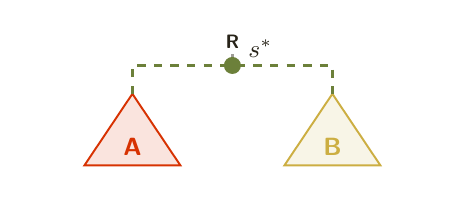
\begin{tikzpicture}[blk]
  \bbox{53}{19}
  \foreach \cx/\c in {13.3/colA, 38.7/colB}{
    \path[fill=\c, fill opacity=.13, draw=\c, line width=.7pt]
      (\cx,8.4) -- ({\cx-6.1},17.5) -- ({\cx+6.1},17.5) -- cycle;}
  \node[ctr, bigA, text=colA] at (13.3,16.2) {A};
  \node[ctr, bigA, text=colB] at (38.7,16.2) {B};
  \draw[colOverlap, dashed, line width=.9pt] (13.3,8.4) -- (13.3,4.8) -- (38.7,4.8) -- (38.7,8.4);
  \draw[nullGrey] (26,4.8) -- (26,3.3);
  \node[ctr, font=\fontsize{7}{8}\bfseries\itshape\selectfont] at (26,2.6) {R};
  \fill[colOverlap] (26,4.8) circle[radius=1.08mm];
  \node[txt, font=\fontsize{9}{10}\bfseries\itshape\selectfont] at (27.9,3.8) {$s^{*}$};
\end{tikzpicture}};
\node[stack={tr1}{1mm}, text width=\innerw, align=center] (cap1)
  {$s^{*}$: node connecting \cA{} and \cB{} in $R$};
% evolutionary search loop (boxes placed relative to each other; block 53 x 16)
\node[stack={cap1}{2mm}] (loop) {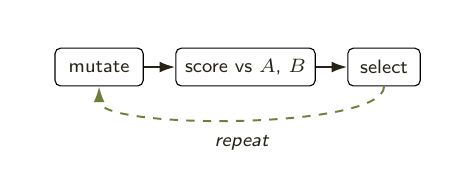
\begin{tikzpicture}[blk]
  \bbox{53}{16}
  \node[procstep, text width=10.5mm, anchor=west] (mut) at (3.4,5) {mutate};
  \node[procstep, text width=17mm, right=4mm of mut] (sc) {score vs $A$, $B$};
  \node[procstep, text width=8.5mm, right=4mm of sc] (sel) {select};
  \draw[->] (mut) -- (sc);
  \draw[->] (sc) -- (sel);
  \draw[->, colOverlap, dashed, line width=.7pt]
    (sel.south) .. controls +(0,5.5) and +(0,5.5) .. (mut.south);
  \node[ctr, font=\fontsize{7}{8}\itshape\selectfont] at ($(mut.south)!.5!(sel.south)+(0,7.6)$) {repeat};
\end{tikzpicture}};
% best score so far (block 53 x 29)
\node[stack={loop}{1mm}] (stair) {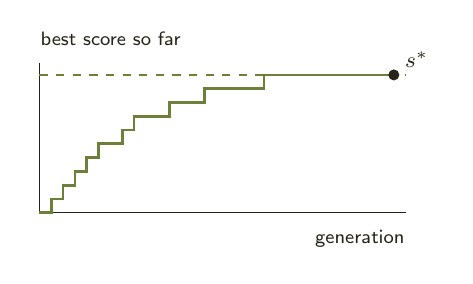
\begin{tikzpicture}[blk]
  \bbox{53}{29}
  \draw[axis] (1.5,23.5) -- (48,23.5);
  \draw[axis] (1.5,23.5) -- (1.5,4.5);
  \node[txt] at (1.5,2.3) {best score so far};
  \node[anchor=base east, inner sep=0pt] at (48,27.4) {generation};
  \draw[colOverlap, line width=1pt] plot[const plot, samples at={0,...,30}]
    ({1.5+45*\x/30},{23.5-17.5*floor(11*(1-exp(-\x/7.8)))/10});
  \draw[colOverlap, dashed, line width=.5pt] (1.5,6) -- (48,6);
  \fill (46.5,6) circle[radius=.7mm];
  \node[txt, font=\fontsize{8}{9}\bfseries\itshape\selectfont] at (47.8,5.0) {$s^{*}$};
\end{tikzpicture}};
\node[outbox, anchor=south] at ([yshift=\padding]c1.south)
  {optimal sequence $s^{*}$\\[1pt] and its \texttt{cmsearch} scores};

  % ================================================================= PANEL 2: median score
\panelhead{c2}{2. Median score}{overlap of A and B, empirical $p$-value}
\vennblock{v2}{c2-s}{2mm}{\adots}
\node[stack={v2}{1mm}, text width=\innerw, align=center] (cap2)
  {overlap $\approx$ median \texttt{cmsearch}$(a_i, B)$};
\node[stack={cap2}{1.6mm}, text width=\innerw, align=left] (t2)
  {Observed: $a_i \leftarrow$ \texttt{cmemit}$(A)$,\\
   $\mobs$ = median \texttt{cmsearch}$(a_i, B)$\\[1.2mm]
   Null: $\mathrm{null}_j = \shuf(a_i)$, $j = 1\ldots n$,\\
   $m_j$ = median \texttt{cmsearch}$(\mathrm{null}_j, B)$};
% histogram of null medians m_j with the observed median as a line (block 53 x 29)
\node[stack={t2}{1.2mm}] (hist) {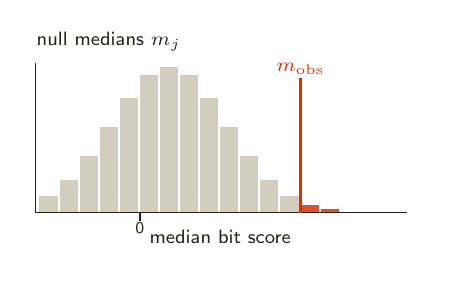
\begin{tikzpicture}[blk]
  \bbox{53}{29}
  \def\hL{1.5}\def\hb{23.5}\def\bw{2.55}
  \foreach \i in {0,...,12}
    \fill[lightGrey] ({\hL+\bw*\i},\hb) rectangle ++({\bw-0.25},{-18.5*exp(-((\i-6)^2)/16.82)});
  \foreach \i in {13,...,15}
    \fill[colA, opacity=.85] ({\hL+\bw*\i},\hb) rectangle ++({\bw-0.25},{-18.5*exp(-((\i-6)^2)/16.82)});
  \draw[axis] (\hL-0.5,\hb) -- ({\hL+18*\bw+0.8},\hb);
  \draw[axis] (\hL-0.5,\hb) -- (\hL-0.5,4.5);

  % zero tick at bin 5, i.e. right at the null peak (bins 0-4 are then negative)
  \draw[axis] ({\hL+5*\bw},\hb) -- ({\hL+5*\bw},{\hb+1});
  \node[ctr, font=\fontsize{6.3}{7.3}\selectfont] at ({\hL+5*\bw},{\hb+2.6}) {0};

  \draw[colA, line width=1pt] ({\hL+13*\bw},6.4) -- ({\hL+13*\bw},\hb);
  \node[ctr, text=colA, font=\fontsize{7}{8}\bfseries\itshape\selectfont] at ({\hL+13*\bw},5.6) {$\mobs$};
  \node[txt] at (\hL-0.5,2.3) {null medians $m_j$};
  \node[ctr] at ({\hL+9*\bw},27.4) {median bit score};
\end{tikzpicture}};
\node[outbox, anchor=south] at ([yshift=\padding]c2.south)
  {median score $\mobs$ and empirical $p$-value\\[1pt] $p = \#\{m_j \ge \mobs\}/(n+1)$};

% ================================================================= PANEL 3: score distribution
\panelhead{c3}{3. Score distribution}{same overlap, compared by KS test}
\vennblock{v3}{c3-s}{2mm}{\adots}
\node[stack={v3}{1mm}, text width=\innerw, align=center] (cap3)
  {$\mobs$ = median \texttt{cmsearch}$(a_i, B)$};
\node[stack={cap3}{1.6mm}, text width=\innerw, align=left] (t3)
  {\texttt{cmsearch}$(a_i, B)$ vs null, whole distribution};
% density and ECDFs with the KS statistic D (block 53 x 45)
\node[stack={t3}{1mm}] (dist) {\begin{tikzpicture}[blk]
  \bbox{53}{45}
  \def\L{3.2}\def\Wd{48}
  % density
  \def\db{17.5}
  \fill[lightGrey, opacity=.75] (\L,\db) --
    plot[domain=-1:1, samples=101] ({\L+\Wd*\x},{\db-\dscale*\nullpdf{\x}}) -- (\L+\Wd,\db) -- cycle;
  \fill[colA, opacity=.28] (\L,\db) --
    plot[domain=-1:1, samples=101] ({\L+\Wd*\x},{\db-\dscale*\obspdf{\x}}) -- (\L+\Wd,\db) -- cycle;
  \draw[nullGrey, line width=.7pt] plot[domain=0:1, samples=101] ({\L+\Wd*\x},{\db-\dscale*\nullpdf{\x}});
  \draw[colA, line width=.7pt]     plot[domain=0:1, samples=101] ({\L+\Wd*\x},{\db-\dscale*\obspdf{\x}});
  \draw[axis] (\L-0.5,\db) -- (\L+\Wd+0.5,\db);
  \draw[axis] (\L-0.5,\db) -- (\L-0.5,3);
  
  \draw[axis] ({\xpos{0.2}},\db) -- ({\xpos{0.2}},{\db+1});
  \node[ctr, font=\fontsize{6.3}{7.3}\selectfont] at ({\xpos{0.2}},{\db+3}) {0};

  \draw[colA, dashed, line width=.7pt] ({\L+\Wd*\xmed},\db) -- ({\L+\Wd*\xmed},3.6);
  \node[ctr, text=colA, font=\fontsize{7}{8}\bfseries\itshape\selectfont] at ({\L+\Wd*\xmed},2.4) {$\mobs$};
  \node[anchor=base east, inner sep=0pt] at (\L+\Wd+0.5,5.0) {density};
  \fill[colA] (\L+0.8,5.3) rectangle ++(1.65,1.65);
  \node[txt] at (\L+3.3,6.8) {observed};
  \fill[nullGrey] (\L+0.8,8.1) rectangle ++(1.65,1.65);
  \node[txt] at (\L+3.3,9.6) {null};
  \node[ctr] at ({\L+\Wd/2},22.5) {bit score};
  % ECDFs
  \def\eb{41}\def\eh{14}
  \draw[nullGrey, line width=1pt] plot[domain=0:1, samples=101] ({\L+\Wd*\x},{\eb-\eh*\nullcdf{\x}});
  \draw[colA, line width=1pt]     plot[domain=0:1, samples=101] ({\L+\Wd*\x},{\eb-\eh*\obscdf{\x}});
  \draw[axis] (\L-0.5,\eb) -- (\L+\Wd+0.5,\eb);
  \draw[axis] (\L-0.5,\eb) -- (\L-0.5,26);

  \node[anchor=base east, inner sep=0pt] at (\L-1.2,\eb+0.6) {0};
  \node[anchor=base east, inner sep=0pt] at (\L-1.2,\eb-\eh+0.6) {1};
  \node[txt] at (\L-0.5,24.4) {cumulative fraction};
  \node[ctr] at ({\L+\Wd/2},44.2) {bit score};
  \pgfmathsetmacro{\yN}{\eb-\eh*\nullcdf{\xD}}
  \pgfmathsetmacro{\yO}{\eb-\eh*\obscdf{\xD}}
  \draw[<->, line width=.8pt, >={Latex[length=1.4mm,width=1.1mm]}]
    ({\L+\Wd*\xD},\yN) -- ({\L+\Wd*\xD},\yO);
  \node[txt, font=\fontsize{9}{10}\bfseries\itshape\selectfont] at ({\L+\Wd*\xD+1.2},{(\yN+\yO)/2+1}) {$D$};
\end{tikzpicture}};
\node[outbox, anchor=south] at ([yshift=\padding]c3.south)
  {median score $\mobs$ and KS statistic $D$ and $p$-value\\[1pt] $D = \max\,|F_{\mathrm{obs}} - F_{\mathrm{null}}|$};

\end{tikzpicture}
\end{document}